\chapter{MT experiment - our model}

\label{chap:mt-exp} % id kapitoly pre prikaz ref

\section{Task description}

\section{Dataset and baseline}

\section{Our model}
self-organisation usage

Pri tvorbe nášho modelu sme uvažovali, ako formulovať chybu konzistencie, ktorá by zahŕňala viac informácie ako v doterajšom modeli. Keďže chyba konzistencie v MT je vyjadrená vzdialenosť vektorov, s rozmerom rovným počtu tried, ide o pomerne málo informácie. Tuna a spol.(2021) vo svojom modeli Binary Mean Teacher modelovali binárnu klasifikáciu prítomnosti objektu na obrázku. V svojom modeli teda nemohli vyjadriť chybu konzistencie pri odozve z intervalu $(0,1)$ pre dve triedy (oproti 10 triedam v CIFAR10) a teda vyjadrili $J(\theta)$ ako MSE na poslednej konvolučnej vrstve použitej architektúry, čiže ešte pred plne prepojenou časťou siete.\footnote{Podobná stratégia sa bežne používa pri transfer learning \cite{weiss2016}, kde sa použije model, ktorý už je dobre natrénovaný na všeobecnej úlohe a jeho plne prepojená vrstva alebo vrstvy sa nahradia novou architektúrou, ktorá modeluje inú úlohu.}

Túto reprezentáciu využijeme aj my a nazývame $x_{conv}$. Predpokladáme, že reprezentácia vstupu po prechode všetkými konvolučnými vrstvami, bude vhodnejšia pre zachytenie rozdielov a podobností medzi obsahom obrazu, než jeho samotná klasifikácia. Náš navrhovaný model ilustrujeme na Obr.\ref{fig:mt-som}.
Ďalej navrhujeme, že pridanie konceptu samoorganizácie môže zlepšiť trénovanie tým, že bude lepšie odzrkadľovať vzdialenosť dát, než pôvodný spôsob počítania $J(\theta)$. Samoorganizáciu zapojíme do počítania $J(\theta)$ tak, že využijeme samoorganizujúcu sa mapu (SOM) \cite{kohonen1990}, ktorú natrénujeme na rozpoznávanie reprezentácií $x_{conv}$ zo študentského aj učiteľského modelu počas danej epochy, keď sa model učí. Potom túto SOM použijeme na počítanie Consistency loss $J(\theta)$.

Samoorganizujúce sa mapy majú vstupnú vrstvu veľkosti vstupného vektora plne prepojenú s nasledujúcou vrstvou, ktorú tvorí mapa neurónov konkrétneho tvaru, napríklad mriežka. V každom neuróne máme parameter siete, vektor veľkosti vstupu, ktorý reprezentuje niečo ako prototyp. Vyjadrením euklidovskej vzdialenosti medzi vstupným neurónov a váhami neurónov vyjadríme víťaza v zmysle najbližšieho neurónu, ktorého váhu potom pri učení posilníme daným vstupom a zároveň posilníme aj jeho okolie. Výsledkom učenia sa SOM je topografická mapa vstupného priestoru, ktorá zachytáva štruktúru a podobnosti v dátach nelineárnym spôsobom.



Označme reprezentácie z poslednej konvolučnej vrstvy študentského a učiteľského modelu ako $x_{conv}$ a $x^\prime_{conv}$. V SOM nájdeme víťazný neurón (winner neuron, best matching unit) pre $x_{conv}$ a $x^\prime_{conv}$, označme $c$ a $c\prime$. Keďže neuróny SOM sú definované ich váhami a tie vlastne reprezentujú polohu tohto neurónu v mnohorozmernom priestore. Potom našim cieľom je, aby $c$ a $c\prime$, predstavujúce vstupné reprezentácie, ktoré vznikli z rovnakého obrázku, boli v tomto priestore čo najbližšie. Preto našu novú chybu konzistencie definujeme ako súčet vzdialenosti víťazov a tiež vzdialenosti víťaza od konvolučnej reprezentácie vstupu. Vzdialenosť dvoch bodov $a, b$ v tomto priestore označíme $d(a, b)$ a teda chybovú funkciu $J(\theta)$ vieme zapísať ako:

\begin{equation}
  J(\theta) = d(c, c\prime) + d(x_{conv}, c) + d(x^\prime_{conv}, c\prime)  
\end{equation}


\begin{figure}
    \centering
    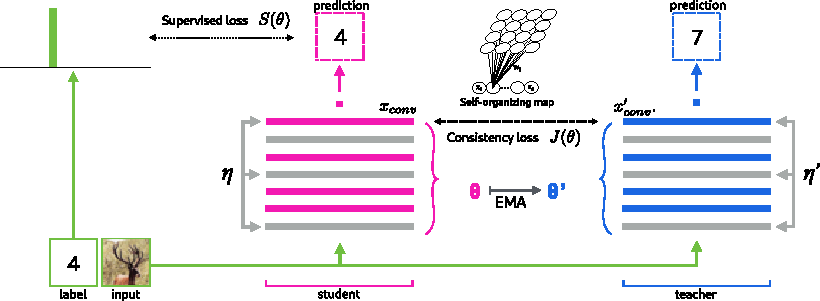
\includegraphics{figs/mean_teacher_som.pdf}
    \caption{Caption}
    \label{fig:mt-som}
\end{figure}

\section{Implementation}

\section{Results}

\section{Discussion}


\begin{figure}
    \centering
    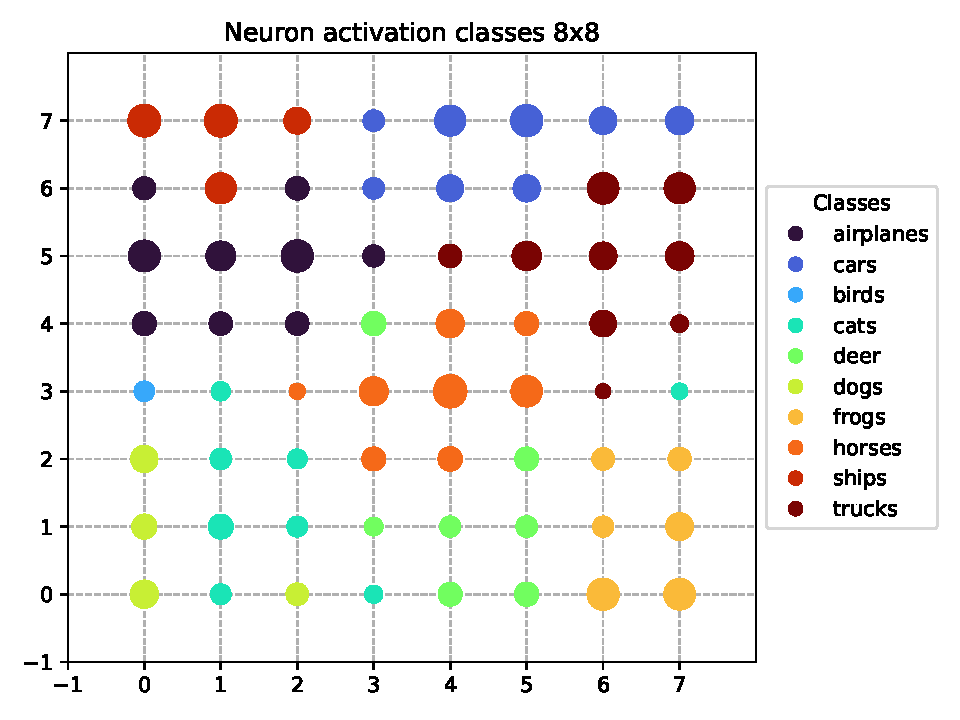
\includegraphics{figs/som-clusters-mt.pdf}
    \caption{Caption}
    \label{fig:enter-label}
\end{figure}


